\documentclass[a4paper,10pt]{article}
\usepackage[utf8]{inputenc}
\usepackage{comment}

\usepackage[
backend=biber,
style=alphabetic,
sorting=ynt
]{biblatex}
\addbibresource{bibliography.bib}   %>>>> bibliography data in bibliography.bib
%\bibliography{bibliography}   %>>>> bibliography data in bibliography.bib
%\bibliographystyle{spiebib}   %>>>> makes bibtex use spiebib.bst


%%%%%%%%%%%%%%%%%%%%%%%%%%%%%%%%%%%%%%%%%%%%%%%%%%%%%%%%%%%%%%%%%%%%%%%%%%%%%%%%
\usepackage{url}
%
\usepackage[breaklinks]{hyperref}
\usepackage{breakurl}

%%%%%%%%%%%%%%%%%%%%%%%%%%%%%%%%%%%%%%%%%%%%%%%%%%%%%%%%%%%%%%%%%%%%%%%%%%%%%%%%
\usepackage{graphicx}
\usepackage{subcaption}
%%%%%%%%%%%%%%%%%%%%%%%%%%%%%%%%%%%%%%%%%%%%%%%%%%%%%%%%%%%%%%%%%%%%%%%%%%%%%%%%

\usepackage[svgnames]{xcolor} % Enabling colors by their 'svgnames'

\usepackage{amsmath}
\usepackage{amsfonts}
\usepackage{amssymb}


%%%%%%%%%%%%%%%%%%%%%%%%%%%%%%%%%%%%%%%%%%%%%%%%%%%%%%%%%%%%%%%%%%%%%%%%%%%%%%%%
\usepackage{amsthm}
\newtheorem{mydef}{Definição}

%%%%%%%%%%%%%%%%%%%%%%%%%%%%%%%%%%%%%%%%%%%%%%%%%%%%%%%%%%%%%%%%%%%%%%%%%%%%%%%%

%opening
\title{Dança, Canais de Comunicação e Novos Paradigmas na Condução}
\author{Fernando Pujaico Rivera, -------- -------- --------}

%%%%%%%%%%%%%%%%%%%%%%%%%%%%%%%%%%%%%%%%%%%%%%%%%%%%%%%%%%%%%%%%%%%%%%%%%%%%%%%%
%%%%%%%%%%%%%%%%%%%%%%%%%%%%%%%%%%%%%%%%%%%%%%%%%%%%%%%%%%%%%%%%%%%%%%%%%%%%%%%%
%%%%%%%%%%%%%%%%%%%%%%%%%%%%%%%%%%%%%%%%%%%%%%%%%%%%%%%%%%%%%%%%%%%%%%%%%%%%%%%%
%%%%%%%%%%%%%%%%%%%%%%%%%%%%%%%%%%%%%%%%%%%%%%%%%%%%%%%%%%%%%%%%%%%%%%%%%%%%%%%%
\begin{document}

\maketitle

\begin{abstract}
Condução
\end{abstract}


%%%%%%%%%%%%%%%%%%%%%%%%%%%%%%%%%%%%%%%%%%%%%%%%%%%%%%%%%%%%%%%%%%%%%%%%%%%%%%%%
%%%%%%%%%%%%%%%%%%%%%%%%%%%%%%%%%%%%%%%%%%%%%%%%%%%%%%%%%%%%%%%%%%%%%%%%%%%%%%%%
%%%%%%%%%%%%%%%%%%%%%%%%%%%%%%%%%%%%%%%%%%%%%%%%%%%%%%%%%%%%%%%%%%%%%%%%%%%%%%%%
\section{Paradigma na dança}

%\begin{mydef}[Paradigma]
%Algo que serve de exemplo ou modelo; padrão \cite{michaelis.uol.com.br}.
%\end{mydef}

\begin{mydef}[Condutor]
Definiremos aqui, condutor como a pessoa encarregada de propôr um movimento, passo ou ação na dança a dóis.
Esta proposta pode ser feita de maneira indicativa, corporal, por indução ou por ausência.
\end{mydef}

\begin{mydef}[Seguidor]
Definiremos aqui, seguidor como a pessoa encarregada, na dança a dóis, 
de  receber a proposta de movimento, passo ou ação;
e realizar uma resposta corporal.
Esta proposta pode chegar de maneira indicativa, corporal, por indução ou por ausência.
\end{mydef}

\begin{mydef}[Paradigma da condução]
Definiremos aqui, o paradigma da condução ou simplesmente condução, 
como o modelo de dança a dóis no qual a informação da proposta do movimento, 
passo ou ação, é transmitida unidirecionalmente desde um condutor ate um seguidor.
Neste modelo de dança o papel do condutor e do seguidor não é intercambiável.


Os autores Maia, M.A.C. e Pereira, V.R. \cite{maia2010danca} explicam que 
essa transmissão de informação acontece por médio dos pontos onde há contato corporal, numa troca de energia constante,
sendo o contato e o adequado nível de pressão importantes para ser bons condutores e seguidores.

Por outro lado, autores como Feitosa J. K. se questionam na suas pesquisas \cite[pp. 24]{Jonas2011},
se o papel do seguidor deve ser apenas resistir à condução do condutor e produzir o charme na dança?
Motivando assim a procura e proposta de outros paradigmas na dança a dois.


%\begin{mydef}[Condução compartilhada]
% https://www.doisrumos.com/single-post/2017/08/07/Voc%C3%AA-sabe-o-que-%C3%A9-Condu%C3%A7%C3%A3o-Compartilhada
%\end{mydef}

%\begin{mydef}[Cocondução]
% \cite{Jonas2011}
%\end{mydef}

%\begin{mydef}[Condução mutua]
%
%\end{mydef}


\end{mydef}

%%%%%%%%%%%%%%%%%%%%%%%%%%%%%%%%%%%%%%%%%%%%%%%%%%%%%%%%%%%%%%%%%%%%%%%%%%%%%%%%
%%%%%%%%%%%%%%%%%%%%%%%%%%%%%%%%%%%%%%%%%%%%%%%%%%%%%%%%%%%%%%%%%%%%%%%%%%%%%%%%
%%%%%%%%%%%%%%%%%%%%%%%%%%%%%%%%%%%%%%%%%%%%%%%%%%%%%%%%%%%%%%%%%%%%%%%%%%%%%%%%
\section{Sistemas de comunicação}
\begin{mydef}[Transmissor]
O transmissor é o encarregado de empacotar a mensagem numa forma apropriada, 
dado que a mensagem diretamente saída da fonte
geralmente não tem as caraterísticas necessárias para ser transmitida eficazmente,
apos este empacotamento o transmissor envia o pacote ao receptor por um canal de comunicação \cite[pp. 10]{ibarra1999principios} \cite[pp. 479]{sawaya2002dicionario}.
\end{mydef}
\begin{mydef}[Receptor]
O receptor recupera o pacote enviado pelo transmissor no canal de comunicação e desempacota a mensagem,
para que esta possa ser usada \cite[pp. 10]{ibarra1999principios} \cite[pp. 389]{sawaya2002dicionario}.
\end{mydef}
\begin{mydef}[Canal de comunicação]
Entre um transmissor e um receptor existe um canal de comunicação que se usa 
para enviar uma sinal ou mensagem de um lugar a outro \cite[pp. 10]{jairo2007analisis} \cite[pp. 364]{lechtaler1999teleinformatica} \cite[pp. 10]{ibarra1999principios}.
Este canal pode enviar informação numa direção ou em ambas, 
ser físico ou lógico, e pode ter fios ou ser sem fios.
\end{mydef}

\subsection{Classificação de canais pelo modo de comunicação}
Podemos classificar um canal de comunicação  
pelo momento em que se efetua a transmissão e a direção; 
entre estes modos temos o ``Simplex channel'', o ``Half duplex channel'' e o 
``Duplex channel'' \cite[pp.60 ]{hura2001data}\cite[pp. 5]{shinde2009computer}.

O \textbf{Simplex channel} denota um médio de comunicação habilitado 
para transmitir dados unicamente numa direção, desde o transmissor ate o receptor 
sendo que estes papeis são designados de maneira fixa 
\cite[pp. 5]{shinde2009computer} \cite[pp. 430]{sawaya2002dicionario} \cite[pp.60 ]{hura2001data}, 
um exemplo disto pode ser visto num sistema de transmissão de rádio onde a emissora 
transmite a música, e o usuário está habilitado só pra receber os dados e escutar, 
sendo este o modo mais simples de implementar uma comunicação,
ver Figura \ref{fig:channelsimplex}. 

O \textbf{Half duplex channel} denota um médio de comunicação onde o canal está
sendo usado numa direção por vez, 
porem esta direção cambia de modo que os papeis de transmissor e receptor são 
intercambiáveis entre os usuários 
\cite[pp. 5]{shinde2009computer}\cite[pp. 208]{sawaya2002dicionario}, ver Figura \ref{fig:channelhalfduplex}. 
Neste modo de comunicação o fim da mensagem numa direção é 
reconhecida pelo receptor, que pode cambiar se precisar a direção da transmissão de dados \cite[pp. 60]{hura2001data}.
É possível observar vários métodos para a troca na direção das mensagens, por exemplo:
\begin{itemize}
\item Em alguns casos existe um tempo de pausa, apos um mensagem ser enviado, 
para esperar a troca de emissor, e a resposta se esta existe \cite[pp. 60]{hura2001data}.
\item Também existem implementações onde se estabelece um protocolo, que define 
métodos para indicar o inicio e o fim de uma mensagem e a troca de emissor. 
Como exemplo disto temos ao protocolo I2C \cite[pp. 82]{gupta2019iot}.
\item O simplesmente por algum método de ação a distancia, 
a direção do canal é cambiada, e este estado é reconhecido pelo novo emissor, 
podendo optar entre enviar uma mensagem, esperar deixando o canal livre, 
ou devolver o sentido do canal a seu estado anterior.
Um exemplo disto seriam os antigos ``walkie-talkie'' onde existia um botão
pra habilitar a mudança de receptor a emissor, e se finalizava a mensagem e pedindo resposta
falando ``over'' (em inglês).

\end{itemize}


O \textbf{Full duplex channel} ou  \textbf{Duplex channel} denota um médio de comunicação onde o
canal permite a transmissão simultânea em ambas as direções \cite[pp. 150]{sawaya2002dicionario},
de modo que não existe o tempo um pausa para a troca do sentido da transmissão, 
como nos canais ``Half duplex'' \cite[pp. 5]{shinde2009computer};
este método de comunicação pode ser implementado fusionando dois ou mais ``simplex channel'' \cite[pp. 60]{hura2001data}.
Um exemplo de um ``Duplex channel'' é a comunicação por celular, 
onde podemos falar e escutar ao mesmo tempo (porem se ambas coisas acontecem ao mesmo tempo, 
o entendimento da mensagem esta limitado pelo cérebro humano e não pelo método de comunicação).

\begin{figure}[ht!]
    \centering
    \begin{subfigure}[b]{0.3\textwidth}
        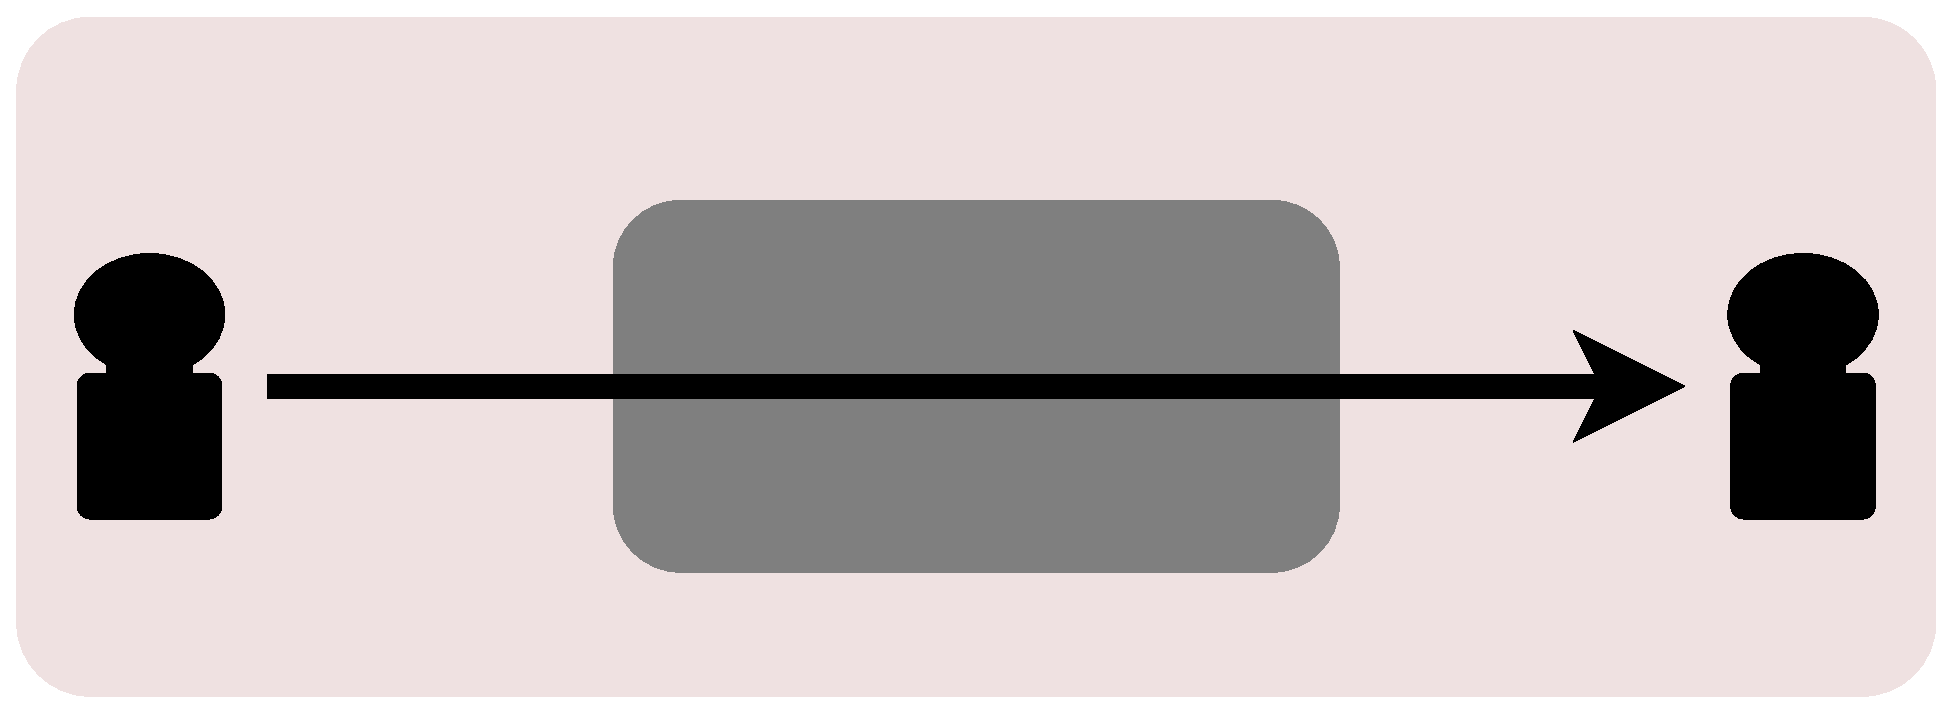
\includegraphics[width=\textwidth]{channel-simplex.eps}
        \caption{Simplex channel}
        \label{fig:channelsimplex}
    \end{subfigure}
    ~ %add desired spacing between images, e. g. ~, \quad, \qquad, \hfill etc. 
      %(or a blank line to force the subfigure onto a new line)
    \begin{subfigure}[b]{0.3\textwidth}
        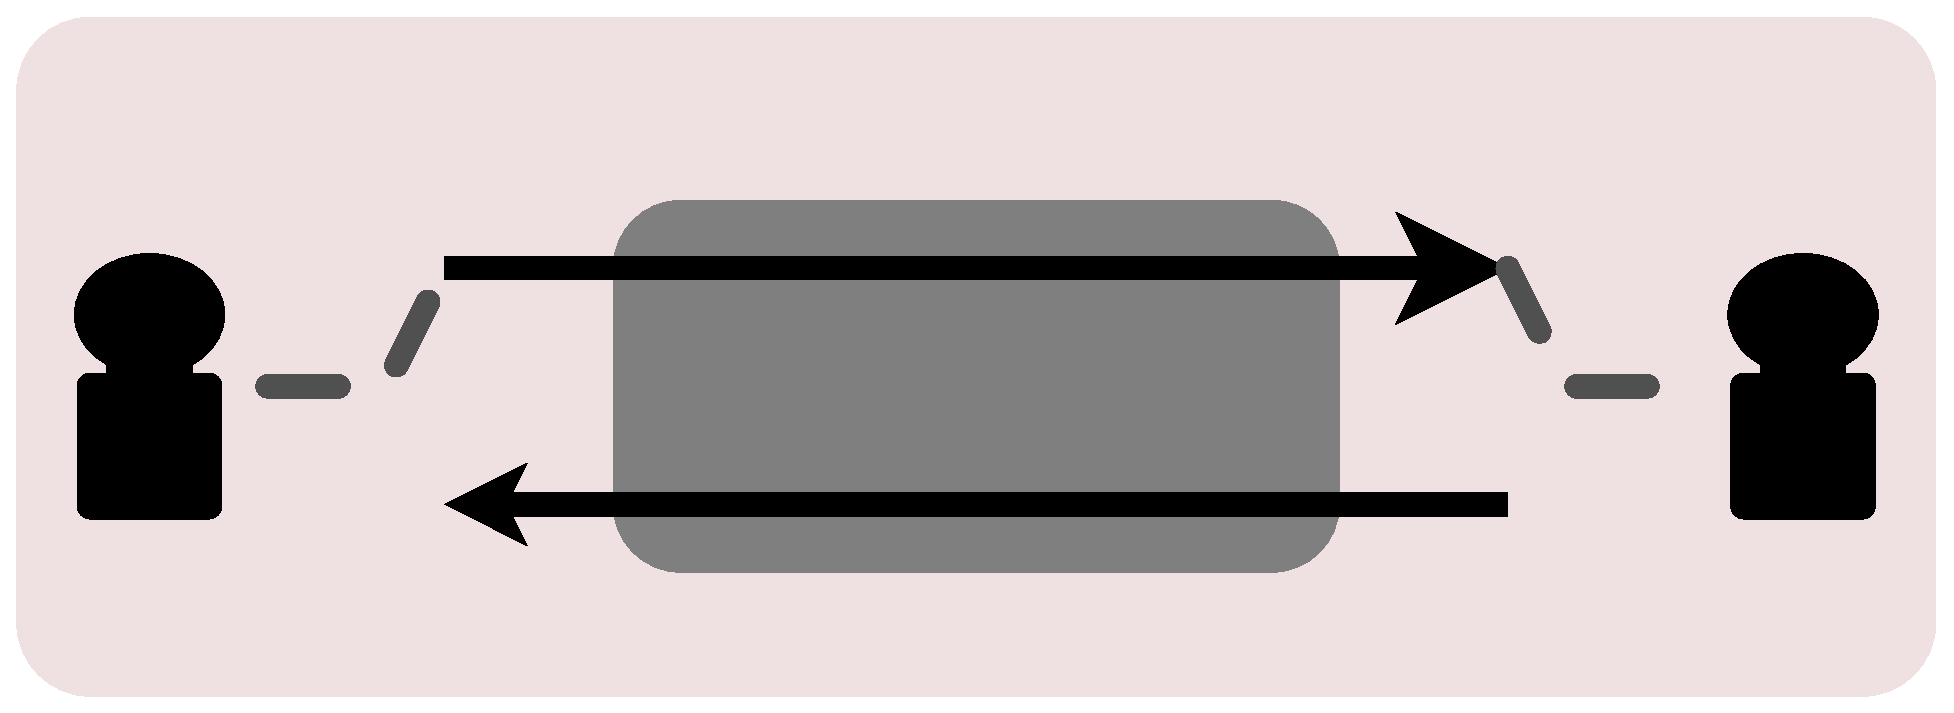
\includegraphics[width=\textwidth]{channel-halfduplex.eps}
        \caption{Half duplex channel}
        \label{fig:channelhalfduplex}
    \end{subfigure}
    ~ %add desired spacing between images, e. g. ~, \quad, \qquad, \hfill etc. 
    %(or a blank line to force the subfigure onto a new line)
    \begin{subfigure}[b]{0.3\textwidth}
        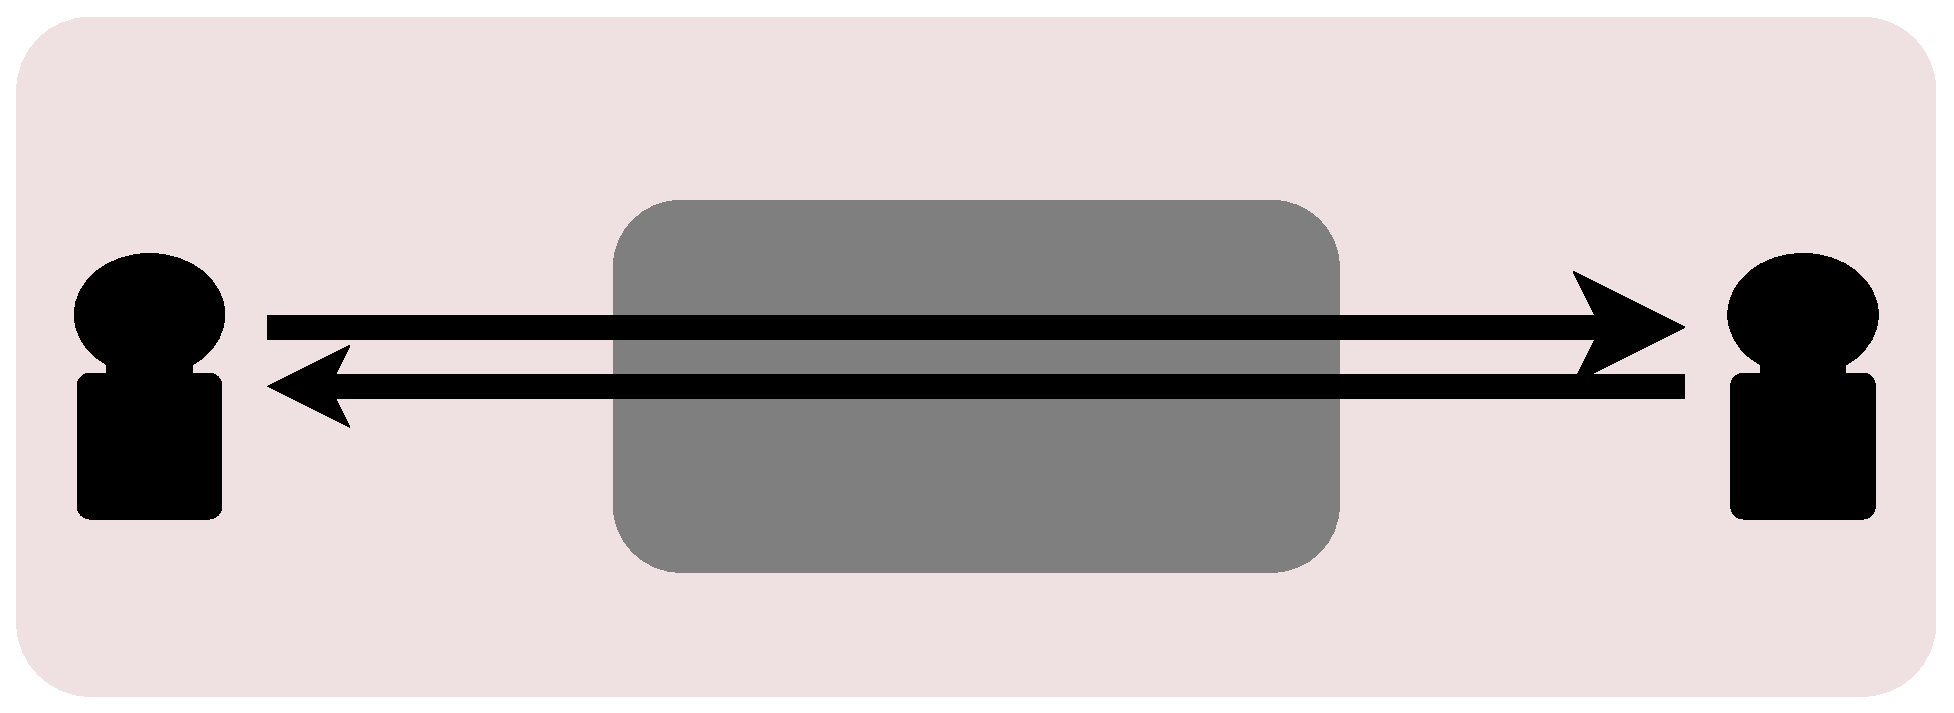
\includegraphics[width=\textwidth]{channel-duplex.eps}
        \caption{Duplex channel}
        \label{fig:channelduplex}
    \end{subfigure}
    \caption{Modos de operação}\label{fig:channeltypes}
\end{figure}


\subsection{Classificação de canais entre físico e lógico}
\subsection{Classificação de canais entre com fio e sem fio}

%%%%%%%%%%%%%%%%%%%%%%%%%%%%%%%%%%%%%%%%%%%%%%%%%%%%%%%%%%%%%%%%%%%%%%%%%%%%%%%%
%%%%%%%%%%%%%%%%%%%%%%%%%%%%%%%%%%%%%%%%%%%%%%%%%%%%%%%%%%%%%%%%%%%%%%%%%%%%%%%%
%%%%%%%%%%%%%%%%%%%%%%%%%%%%%%%%%%%%%%%%%%%%%%%%%%%%%%%%%%%%%%%%%%%%%%%%%%%%%%%%
\section{Relação entra a dança e um sistema de comunicação}
Tabela \ref{tab:table1}
\begin{table}[h!]
  \begin{center}
    \caption{Your first table.}
    \label{tab:table1}
    \begin{tabular}{|l|p{6cm}|} % ff
    \hline
      Modos de transmissão & Paradigma na dança \\ \hline \hline
      Simplex channel & Condução (no sentido clássico)  \\ \hline
      Half duplex channel & Condução com troca de condutor durante a comunicação\\ \hline
      Duplex channel & Condução acontecendo em ambos sentidos ao mesmo tempo \\ \hline
    \end{tabular}
  \end{center}
\end{table}

%%%%%%%%%%%%%%%%%%%%%%%%%%%%%%%%%%%%%%%%%%%%%%%%%%%%%%%%%%%%%%%%%%%%%%%%%%%%%%%%
%%%%%%%%%%%%%%%%%%%%%%%%%%%%%%%%%%%%%%%%%%%%%%%%%%%%%%%%%%%%%%%%%%%%%%%%%%%%%%%%
%%%%%%%%%%%%%%%%%%%%%%%%%%%%%%%%%%%%%%%%%%%%%%%%%%%%%%%%%%%%%%%%%%%%%%%%%%%%%%%%
\section{Quando mais de uma pessoa envia dados}

Quando duas pessoas na dança optam por tomar o papel de condutor, 
e enviar dados pelo canal de comunicação sem nenhum protocolo;
acontece então uma colisão e destruição\footnote{Se o objetivo era criar algo novo, então não é destruição, 
porem a isto não pode-se chamar uma transmissão de mensagem, 
pois as mensagens originais foram destruídas, isto é uma co-criação.} 
da informação, de forma aleatória,
dependendo do momento de uso do canal de comunicação que faça cada uma das partes. 
É chamado de destruição, porque ambos mensagens originais são perdidos,
pra criar um novo que contem parte da informação de ambos mensagens,
porem recuperar a totalidade da informação de qualquer destes dois mensagens é 
impossível sem nenhum tipo de redundância na mensagem, e métodos de decodificação,
pois atingimos um limite teórico estabelecido pelo 
teorema de Shannon\footnote{Ou teorema de Shannon-Hartley, teorema de codificação para canais com ruido.} 
\cite[pp. 22]{vanLint2012introduction}. 


Para entender este processo de interferência, 
criaremos um exemplo onde  simplificaremos e modelaremos a duas pessoas, 
os dançarinos  $C$ e $S$;
que serão representados, como fontes discretas sem memoria, que geram símbolos binários de forma aleatória,
é dizer fontes binarias \cite[pp. 90]{reza2012introduction}.

A \textbf{pessoa C} tem uma dança, com um alfabeto composto unicamente por dois tipos de ações,
$A_0$ e $A_1$, e executa uma ou outra ação de forma aleatória a cada tempo 
(não necessariamente o tempo do compasso), realizando só uma ação por vez. 
De modo que os movimentos ou passos executados por esta pessoa, 
são a união temporal, uma apos de outra, destas ações; 
exemplo, um passo pode ser $A_1 A_0 A_1 A_1 A_0 A_1$.
A probabilidade de que a pessoa execute a ação $A_1$ para um tempo qualquer é
igual a $p_c$, é dizer: $P(C=A_1)\equiv p_c$  


A \textbf{pessoa S} se define de forma similar que a pessoa C, e com o mesmo alfabeto de ações;
porem, com a diferencia de que a probabilidade de que a pessoa S, 
execute a ação $A_1$ para um tempo qualquer é
igual a $p_s$, é dizer: $P(S=A_1)\equiv p_s$.
isto é, só se diferencia de C pela probabilidade com a que executa as ações.


\begin{mydef}[Entropia binaria]
A Entropia binaria de uma fonte, 
é uma forma da medida da informação que esta produz por cada simbolo enviado. 
Para o caso de uma fonte binaria $A$, 
a entropia binaria se define como $H(A)$;
se conhecemos a probabilidade $p$ de um dos símbolos da fonte $A$, 
podemos usar outra forma de escrita equivalente, como $h_b(p)$ \cite[pp. 90]{reza2012introduction} \cite[pp. 5]{cover2012elements},
\begin{equation}
H(A)\equiv h_b(p)=-p~log_2(p)-(1-p)log_2(1-p).
\end{equation}
\end{mydef}


\section{Analisis de conceitos}

\subsection{vc concorda que, quem recebe a condução não pode conduzir ou interferir?}
No paradigma na dança com transmissão de mensagem de forma unidirecional com emissor fixo (paradigma da condução), 
não pode, pois atrapalha o fluxo de informação. 
Porem sim se deseja trabalhar com um fluxo bidirecional de dados, 
atualmente outros paradigmas da dança tem se desenvolvendo e estudando. 
Mas estos são outros paradigmas na dança;
se você aceita usar o paradigma da condução, 
tem que seguir as regras para obter um bom fluxo de informação. 
A analises do problema fica fácil se fazemos uma metáfora: 
Pergunta: Se converso com um falante de espanhol tenho que falar em espanhol, ou posso falar em português as vesses?. 
Resposta: poder falar português pode, porem vc vai gerar erros no fluxo de informação, 
se decidiu conversar em espanhol, fale espanhol, 
ou avise que deseja falar em português ou que deseja falar uma mistura.
%%%%%%%%%%%%%%%%%%%%%%%%%%%%%%%%%%%%%%%%%%%%%%%%%%%%%%%%%%%%%%%%%%%%%%%%%%%%%%%%
%%%%%%%%%%%%%%%%%%%%%%%%%%%%%%%%%%%%%%%%%%%%%%%%%%%%%%%%%%%%%%%%%%%%%%%%%%%%%%%%
%%%%%%%%%%%%%%%%%%%%%%%%%%%%%%%%%%%%%%%%%%%%%%%%%%%%%%%%%%%%%%%%%%%%%%%%%%%%%%%%
\section{Conclusões}
Nas nossas pesquisas sobre novos paradigmas da condução, seja compartilhando, 
co-conduzindo ou produzindo a dança de forma mutua, 
tenho achado muito material não 
acadêmico\footnote{Postagens em blogs com temas relativos a dança.} 
focando a importância destes novos paradigmas na dança, 
numa luta social sobre o papel das pessoas na dança seguindo o sexo.
Acho que é um error promover ou divulgar estes novos paradigmas na dança 
como um método para a liberação da opressão do condutor escolhido por seu sexo;
esse conflito nasce só de uma postura ideológica. 
Pois, se só isso fosse o problema, 
bastaria com empoderar as pessoas que atualmente não usam, 
ou se planteiam usar, esse papel na sociedade, 
a tomar ou pedir o papel de condutor nas danças, 
dado que atualmente não existe nenhuma norma que o proíba,
ou alguma instituição que regule ou sancione este comportamento,
e que exija em caráter mandatório o papel de um individuo na condução seguindo o sexo,
isso ate agora era só uma convenção social, 
dado que o único método de comunicação conhecido na dança era a comunicação unidirecional de emissor fixo;
consequentemente um individuo devia tomar o papel de condutor e outro de seguidor;
de modo que foi usado o padrão cultural da época, da criação das danças, 
para escolher o papel de cada pessoa na dança a dois,
criando deste jeito um estereotipo funcional. 
Assim, atualmente o papel de condutor está habilitado para toda pessoa que se interesse em 
cultivá-lo e aprendê-lo. 
Pelo qual se promovemos o valor destes novos paradigmas na dança baseando-nos na luta social e sexual, 
estos não teriam sentido de existir, 
pois nenhuma pessoa na sociedade atual está proibida de tomar o papel de condutor.

Por outo lado, a um nível técnico e fácil perceber que na dança, além da comunicação 
unidirecional de emissor fixo  (paradigma da condução),
existem alguns outros modos de comunicação pouco explorados ate agora,
como a comunicação com troca de emissor, 
usando o canal de transmissão em um sentido por vez,
e também a comunicação bidirecional com mensagens indo de um lado a outro em simultâneo.
Ate agora a porta do conhecimento e pesquisa estava unicamente aberta para a 
comunicação unidirecional de emissor fixo, 
sendo que as outras duas portas restantes antes mencionadas estão ainda pouco 
exploradas e com infinitas possibilidades a descobrir e pesquisar; 
na nossa humilde opinião, este é o verdadeiro valor destes novos paradigmas na dança. 

%%%%%%%%%%%%%%%%%%%%%%%%%%%%%%%%%%%%%%%%%%%%%%%%%%%%%%%%%%%%%%%%%%%%%%%%%%%%%%%%
%%%%%%%%%%%%%%%%%%%%%%%%%%%%%%%%%%%%%%%%%%%%%%%%%%%%%%%%%%%%%%%%%%%%%%%%%%%%%%%%
%%%%%%%%%%%%%%%%%%%%%%%%%%%%%%%%%%%%%%%%%%%%%%%%%%%%%%%%%%%%%%%%%%%%%%%%%%%%%%%%
%%%%%%%%%%%%%%%%%%%%%%%%%%%%%%%%%%%%%%%%%%%%%%%%%%%%%%%%%%%%%%%%%%%%%%%%%%%%%%%%

\medskip
 
\printbibliography

\end{document}
